\documentclass{article}
\usepackage{iclr2026_conference,times}
\usepackage{hyperref}
\usepackage{url}
\usepackage{booktabs}
\usepackage{graphicx}
\usepackage{amsmath}
\usepackage{amssymb}
\usepackage{microtype}
\usepackage{xcolor}
\usepackage{colortbl}

% ──────────────────────────────────────────────────────────────────────────────
\title{Co-Activation Aware Expert Pruning for\\
Mixture-of-Experts Models}

% Keep commented for anonymous submission.
\iclrfinalcopy

\author{Jiahao Chen \\
Georgia Institute of Technology \\
\texttt{jchen3392@gatech.edu}
\And
Jane Yijun Sun \\
Georgia Institute of Technology \\
\texttt{ysun713@gatech.edu}
}

\newcommand{\fix}{\marginpar{FIX}}
\newcommand{\new}{\marginpar{NEW}}

\begin{document}
\maketitle

% ── Admin fields ───────────────────────────────────────────────────────────────
\paragraph{Collaboration and Team Member Contributions.}
Jane Yijun Sun conducted the literature review, led ideas on the
research direction, and contributed to the writing of this report.
Jiahao Chen designed the methodology, and  conducted experiments.
Both members jointly participated in discussion and iterative refinement throughout
the project.

% ── Abstract ──────────────────────────────────────────────────────────────────
\begin{abstract}
Mixture-of-Experts (MoE) models achieve computational efficiency by routing each token
to a sparse subset of expert networks, but the large number of experts creates
memory and computational overhead.
We investigate whether co-activation patterns in routing decisions can identify experts that are redundant or harmful, enabling 
systematic expert pruning in MoE models.
Building on the expert collaboration analysis from Occult~\citep{luo2025occult},
we construct co-activation matrices from routing statistics and develop structural
metrics (utilization, redundancy, centrality) to rank experts for pruning.
Our experiments on TinyMixtral-4x248M-MoE so far finds that structural
metrics based on co-activation alone do not reliably predict pruning impact.
However, sensitivity analysis shows that one expert (Expert~2) is
\emph{harmful} across all 12 layers of our TinyMixtral model ---disabling it \emph{improves} perplexity by
80--160 points.
These results suggest that co-activation analysis theoretically could have room to identify redundant
and harmful experts, opening new directions for MoE model compression.
\end{abstract}

% ── 1. Introduction ───────────────────────────────────────────────────────────
\section{Introduction}

Sparse Mixture-of-Experts architectures enable large language models to scale parameter
counts without proportionally increasing per-token computation, by conditionally
activating only a small subset of expert feed-forward networks per
token~\citep{shazeer2017outrageously,fedus2022switch}.
However, maintaining a large pool of experts creates memory pressure and computational
overhead, particularly during inference where all expert weights must be stored even
though only a fraction are used per token.

Our initial proposal focused on \emph{hardware-aware expert
placement}---using co-activation patterns to optimize expert execution order and
exploit GPU memory hierarchy for faster inference.
However, during our investigation of co-activation structure, we identified a more
fundamental question: \emph{can co-activation patterns reveal which experts are
redundant or even harmful, enabling systematic expert pruning?}

This shift in focus is motivated by three observations:
(1)~Co-activation analysis reveals not just locality but also structural redundancy---
experts that always fire together may be candidates for merging or removal.
(2)~Expert pruning directly reduces model size and memory footprint, providing
benefits beyond execution optimization.
(3)~Understanding which experts can be safely removed informs both pruning and
placement strategies.

\textbf{Scientific question.}
Can co-activation-based structural metrics predict which experts can be pruned
with minimal quality degradation in MoE models?

We pursue this question by: (1)~constructing expert collaboration matrices from
routing statistics, (2)~computing structural metrics including utilization,
redundancy, and graph centrality, (3)~comparing structural predictions against
ground-truth sensitivity measurements, and (4)~analyzing the surprising case of
harmful experts that improve model quality when removed.

% ── 2. Related Work ───────────────────────────────────────────────────────────
\section{Related Work}

\paragraph{MoE routing and architecture.}
Sparse top-$k$ gating for language modeling was introduced by~\citet{shazeer2017outrageously}
and scaled further in Switch Transformer~\citep{fedus2022switch}, which simplified
routing to top-1 and identified load imbalance as the central practical challenge.
Recent work has explored fine-grained expert segmentation~\citep{deepseek2024} and
shared experts to improve routing patterns.
Our work analyzes routing decisions to identify pruning opportunities rather than
modifying the routing mechanism itself.

\paragraph{Expert placement and communication.}
Occult~\citep{luo2025occult} models expert co-activation frequency to place
collaborating experts on the same GPU, reducing cross-device communication.
Our work repurposes this co-activation analysis for a different goal: identifying
experts that can be removed entirely.
We use the collaboration matrix not for placement optimization but as input to
structural metrics that predict pruning candidates.

\paragraph{Model pruning and compression.}
Neural network pruning has a long history, from early magnitude-based weight
pruning to modern structured pruning approaches.
For MoE models, pruning can operate at the expert level---removing entire expert
networks rather than individual weights.
This coarse-grained approach preserves the MoE routing structure while reducing
the expert pool size.
Our contribution is using co-activation patterns, rather than weight magnitudes
or gradients, to guide expert-level pruning decisions.
\citet{he2024demystifying} proposed a unified compression framework
combining expert-level weight pruning, quantization, and structured
module removal, establishing that utilization and weight magnitude
are the dominant signals used in existing work.

% ── 3. Approach ───────────────────────────────────────────────────────────────
\section{Approach}

\subsection{Expert Collaboration Matrix}

We profile routing decisions by forwarding a calibration corpus through each MoE layer
and recording the top-$k$ selected experts per token.
For a layer with $E$ experts, we define the collaboration matrix
$C \in \mathbb{Z}_{\geq 0}^{E \times E}$:
\begin{equation}
    C_{ij} \;=\; \sum_{t=1}^{T}
        \mathbf{1}\!\left[i \in \mathrm{top\text{-}}k(t)\right]
        \cdot
        \mathbf{1}\!\left[j \in \mathrm{top\text{-}}k(t)\right],
        \quad i \neq j
    \label{eq:collab}
\end{equation}
where $T$ is the number of tokens profiled.
High $C_{ij}$ means experts $i$ and $j$ are frequently co-selected.
Unlike prior work that uses $C$ for placement, we use it to derive pruning metrics.
Figure~\ref{fig:coactivation} shows an example co-activation matrix from Layer~0.

\begin{figure}[h]
\centering
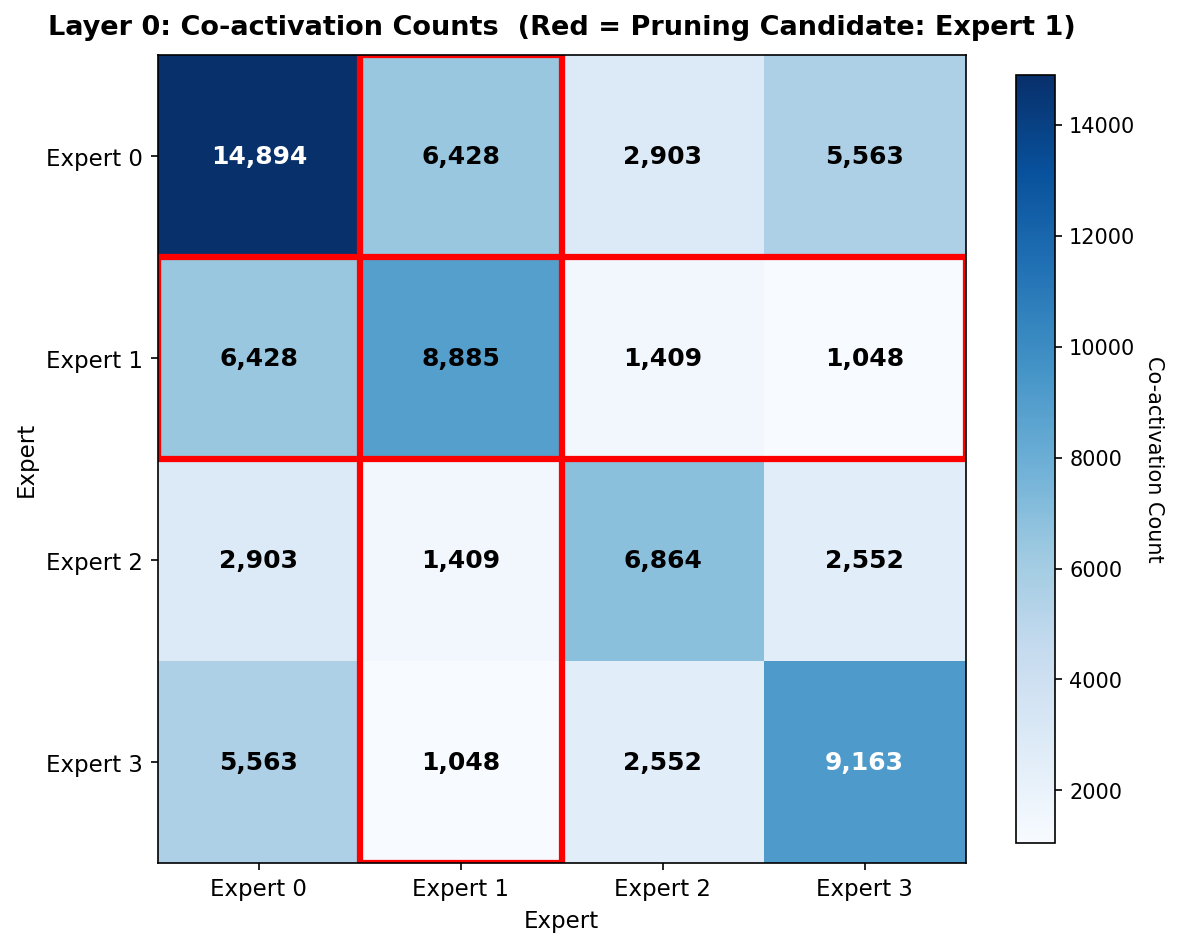
\includegraphics[width=0.5\textwidth]{plots/layer_0_coactivation.png}
\caption{Expert co-activation matrix for Layer~0 of TinyMixtral. Each cell shows
the number of tokens where both experts were selected by top-2 routing.
The matrix reveals which expert pairs frequently collaborate, informing
redundancy and centrality metrics.}
\label{fig:coactivation}
\end{figure}

\subsection{Structural Pruning Metrics}

We compute three categories of metrics from the collaboration matrix:

\paragraph{Utilization.}
Expert utilization measures selection frequency:
\begin{equation}
    \text{Utilization}_i = \frac{\text{times expert } i \text{ selected}}{\text{total routing decisions}}
\end{equation}
Low-utilization experts are natural pruning candidates as they contribute to fewer tokens.

\paragraph{Redundancy.}
We define redundancy as the maximum conditional co-activation probability:
\begin{equation}
    \text{Redundancy}_i = \max_{j \neq i} P(\text{expert } j \text{ fires} \mid \text{expert } i \text{ fires})
\end{equation}
High redundancy suggests expert $i$'s computation may be ``covered'' by a partner expert.

\paragraph{Graph Centrality.}
Treating $C$ as an adjacency matrix, we compute eigenvector centrality to identify
hub experts that collaborate broadly:
\begin{equation}
    \mathbf{c} = \lambda^{-1} C \mathbf{c}
\end{equation}
where $\mathbf{c}$ is the centrality vector and $\lambda$ is the dominant eigenvalue.
Low-centrality experts are peripheral and may be safer to remove.

\paragraph{Structural Score.}
We combine metrics into a single pruning score:
\begin{equation}
    \text{Score}_i = \alpha (1 - \text{Utilization}_i) + \beta \cdot \text{Redundancy}_i + \gamma (1 - \text{Centrality}_i)
\end{equation}
with $\alpha=0.3$, $\beta=0.4$, $\gamma=0.3$ (these values are subject to later refinements).
Higher scores indicate better pruning candidates according to structural metrics.

\subsection{Expert Masking}

To evaluate pruning impact without modifying model weights, we implement \emph{expert masking}.
For each disabled expert, we hook the router's forward pass and:
\begin{enumerate}
    \item Zero out routing weights for tokens assigned to disabled experts
    \item Renormalize remaining weights to sum to 1
\end{enumerate}
This soft-disabling approach allows rapid evaluation of any pruning configuration.

\subsection{Sensitivity Analysis}

As ground truth, we measure per-expert sensitivity:
\begin{equation}
    \text{Sensitivity}_{l,e} = \text{PPL}(\text{model with expert } e \text{ disabled in layer } l) - \text{PPL}(\text{baseline})
\end{equation}
Positive sensitivity indicates the expert is important (removal hurts quality).
Negative sensitivity indicates the expert is \emph{harmful} (removal helps quality).

\subsection{Baselines}

We compare our structural-score-based pruning against the following baselines:

\paragraph{No pruning (primary baseline).}
The unpruned model serves as our primary baseline, establishing the quality ceiling.
All pruning methods are evaluated by their perplexity increase relative to this baseline.

\paragraph{Planned baselines (in progress).}
We are implementing additional baselines for the final report:
\begin{itemize}
    \item \textbf{Random pruning:} Remove experts uniformly at random
    \item \textbf{Utilization-based pruning:} Remove least-frequently-selected experts first
    \item \textbf{Magnitude-based pruning:} Remove experts with smallest weight norms first
\end{itemize}
These will allow us to determine whether co-activation-based metrics outperform
simpler heuristics.

\subsection{Code}

All experiment code is implemented by us and available at
\url{https://github.com/JHCuc3m/MoE-Place}.
The codebase includes:
\begin{itemize}
    \item Co-activation statistics collection via PyTorch forward hooks
    \item Structural metric computation (utilization, redundancy, centrality)
    \item Expert masking via router weight modification
    \item Sensitivity analysis pipeline
    \item Visualization tools for co-activation matrices and sensitivity heatmaps
\end{itemize}
We use HuggingFace \texttt{transformers}~\citep{wolf2020huggingface} for model loading
and \texttt{datasets} for data loading.
All other analysis code is written from scratch.

% ── 4. Experiments ────────────────────────────────────────────────────────────
\section{Preliminary Experiments \& Results}

\subsection{Experimental Setup}

\paragraph{Model.}
We use TinyMixtral-4x248M-MoE~\citep{tinymixtralhf}, a pretrained Mixtral-style model with:
12 transformer layers, 4 experts per layer (48 total), top-2 routing, and
approximately 1B parameters.
Using a pretrained model ensures realistic routing patterns.

\paragraph{Data.}
We use WikiText-2~\citep{merity2017pointer} for both calibration and evaluation:
\begin{itemize}
    \item \textbf{Calibration:} 128 samples from training split (19,903 tokens) for co-activation collection
    \item \textbf{Evaluation:} Full test split (663,040 tokens) for perplexity measurement
\end{itemize}

\paragraph{Hardware.}
Experiments run on NVIDIA H100 80GB GPUs via Georgia Tech PACE cluster, using
PyTorch 2.6 and CUDA 12.4.

\paragraph{Evaluation method.}
We evaluate model quality using \textbf{perplexity} on the WikiText-2 test set.
Lower perplexity indicates better language modeling performance.
For pruning evaluation, we report the perplexity increase relative to the unpruned
baseline---positive values indicate quality degradation, while negative values
(observed for harmful experts) indicate quality improvement.

\subsection{Baseline and Structural Score Pruning}

Our baseline (unpruned) model achieves \textbf{800.38 perplexity} on WikiText-2 test.

The structural score ranking identified \textbf{Layer~0, Expert~1} as the top
pruning candidate (score: 0.789) due to:
\begin{itemize}
    \item High redundancy: 72.3\% (frequently co-activates with another expert)
    \item Moderate-low utilization: 22.3\%
    \item Not the central hub (Expert~0 has highest centrality at 0.643)
\end{itemize}

\paragraph{Result.}
Pruning Layer~0, Expert~1 increased perplexity to \textbf{890.15} (+89.77, +11.2\%).
Despite 72\% redundancy, removal caused significant degradation.

\subsection{Sensitivity Analysis}

We conducted full sensitivity analysis, measuring perplexity impact of disabling
each of the 48 experts individually.
Table~\ref{tab:sensitivity} shows results for all layers.

\begin{table}[h]
\centering
\caption{Expert sensitivity (PPL increase when disabled). Negative values indicate
removal \emph{improves} quality. Bold indicates most sensitive expert per layer.}
\label{tab:sensitivity}
\small
\begin{tabular}{cccccl}
\toprule
\textbf{Layer} & \textbf{Expert 0} & \textbf{Expert 1} & \textbf{Expert 2} & \textbf{Expert 3} & \textbf{Most Sensitive} \\
\midrule
0  & \textbf{+188.2} & +89.8  & \cellcolor{blue!15}$-$155.7 & +87.9  & Expert 0 \\
1  & +31.7  & \textbf{+44.3}  & \cellcolor{blue!15}$-$79.1  & +38.5  & Expert 1 \\
2  & +18.1  & +41.1  & \cellcolor{blue!15}$-$80.9  & \textbf{+47.9}  & Expert 3 \\
3  & +22.0  & \textbf{+67.2}  & \cellcolor{blue!15}$-$110.6 & +60.2  & Expert 1 \\
4  & +43.6  & \textbf{+115.0} & \cellcolor{blue!15}$-$152.5 & +50.0  & Expert 1 \\
5  & +36.1  & \textbf{+101.3} & \cellcolor{blue!15}$-$162.2 & +60.8  & Expert 1 \\
6  & +55.6  & +58.3  & \cellcolor{blue!15}$-$156.9 & \textbf{+91.7}  & Expert 3 \\
7  & +36.6  & +105.3 & \cellcolor{blue!15}$-$163.0 & \textbf{+108.9} & Expert 3 \\
8  & +42.7  & +43.2  & \cellcolor{blue!15}$-$94.3  & \textbf{+80.9}  & Expert 3 \\
9  & \textbf{+54.5}  & +29.2  & \cellcolor{blue!15}$-$84.7  & +51.7  & Expert 0 \\
10 & \textbf{+123.5} & +14.5  & \cellcolor{blue!15}$-$107.6 & +50.5  & Expert 0 \\
11 & \textbf{+190.4} & $-$1.2   & \cellcolor{blue!15}$-$89.1  & +32.1  & Expert 0 \\
\bottomrule
\end{tabular}
\end{table}


\begin{figure}[h]
\centering
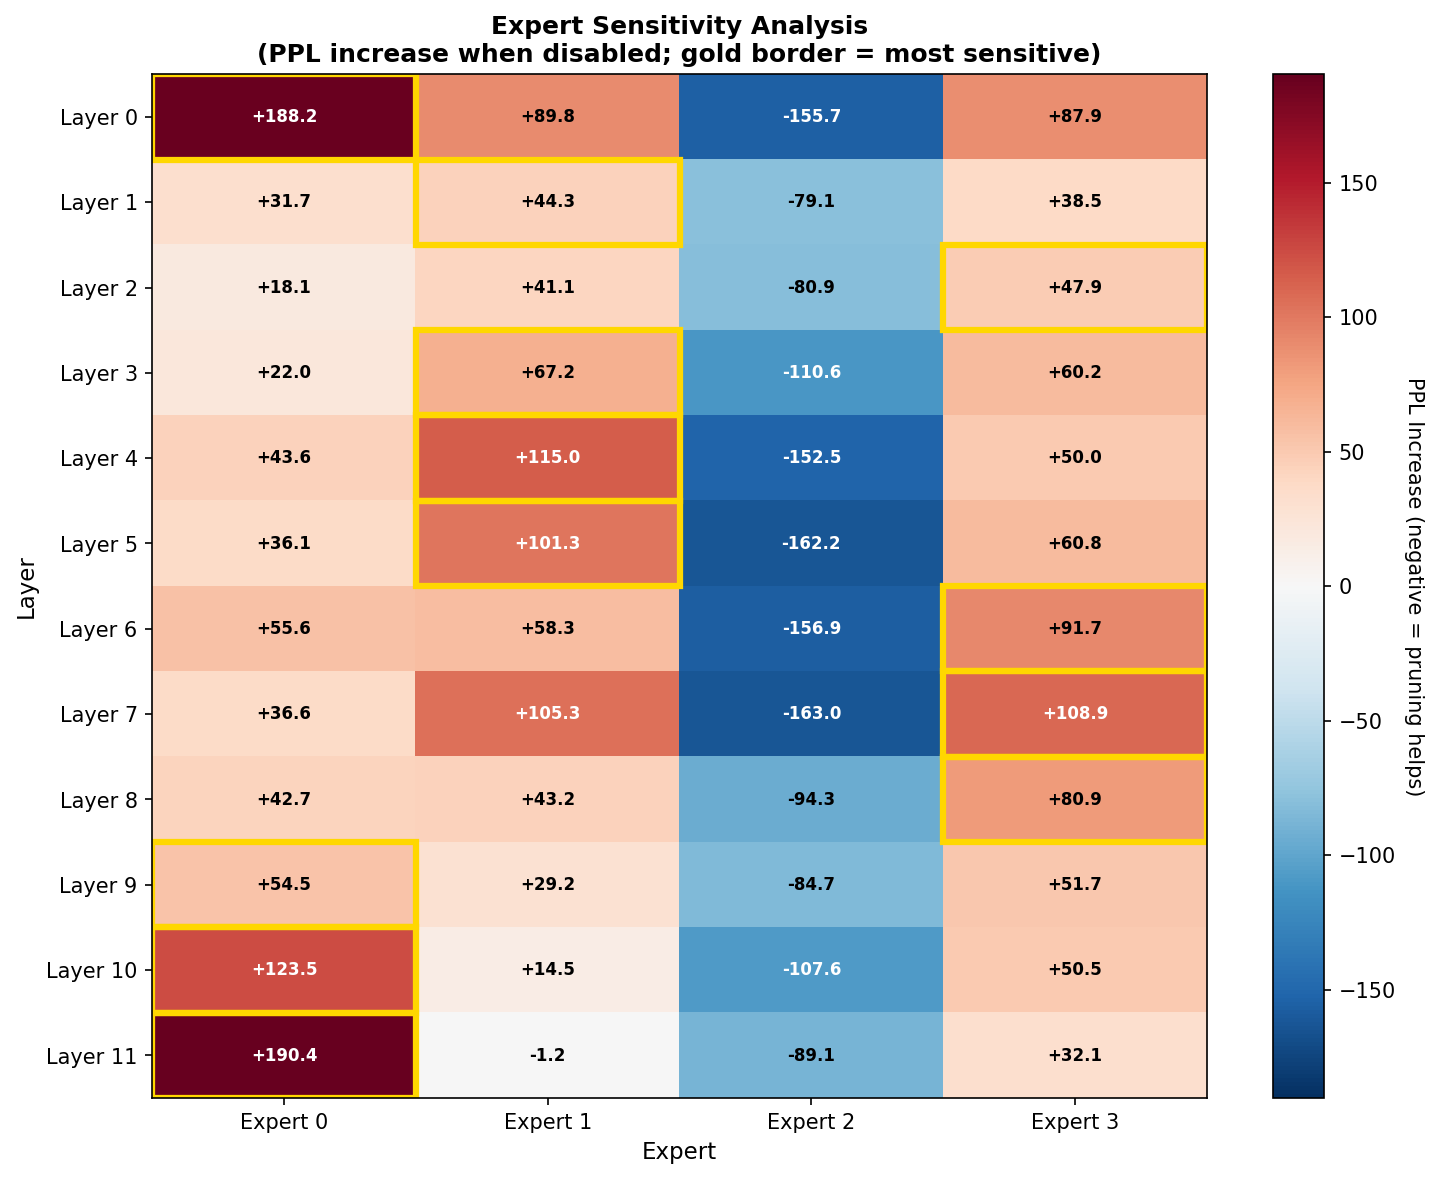
\includegraphics[width=0.65\textwidth]{plots/sensitivity_heatmap.png}
\caption{Sensitivity heatmap showing PPL increase when each expert is disabled.
Red indicates high sensitivity (important experts), blue indicates negative
sensitivity (harmful experts). Expert~2 is harmful across all 12 layers.
Gold borders mark the most sensitive expert per layer.}
\label{fig:sensitivity}
\end{figure}

\subsection{Key Findings}

\paragraph{Finding 1: Expert~2 is harmful across all layers.}
The most striking result is that \textbf{Expert~2 shows negative sensitivity in
all 12 layers} (range: $-$79 to $-$163).
Disabling Expert~2 \emph{improves} perplexity, suggesting it learned harmful or
noisy patterns during pretraining.
This was completely missed by structural metrics, which ranked Expert~2 in the
middle (ranks 25--48 out of 48).

\paragraph{Finding 2: Edge layers are critical.}
Layers 0 and 11 show the highest sensitivity to expert removal.
Expert~0 at these edge layers has sensitivity of +188 and +190, making it the
most critical expert in the model.
Middle layers (1--10) show more moderate sensitivity (+44 to +123).

\paragraph{Finding 3: Structural scores do not predict sensitivity.}
Table~\ref{tab:comparison} compares structural predictions against actual sensitivity.

\begin{table}[h]
\centering
\caption{Comparison of structural score ranking vs.\ actual sensitivity.}
\label{tab:comparison}
\begin{tabular}{lccc}
\toprule
\textbf{Expert} & \textbf{Structural Rank} & \textbf{Structural Score} & \textbf{Actual Sensitivity} \\
\midrule
Layer 0, Expert 1 & 1 (prune first) & 0.789 & +89.8 (important) \\
Layer 0, Expert 2 & 25 (middle)     & 0.600 & $-$155.7 (harmful!) \\
Layer 0, Expert 0 & 37 (keep)       & 0.012 & +188.2 (critical) \\
\bottomrule
\end{tabular}
\end{table}

The structural score correctly identified Expert~0 as important (low score = keep),
but failed to identify Expert~2 as the best pruning target.
High redundancy (72\%) did not translate to safe removal for Expert~1.

\paragraph{Finding 4: Redundancy $\neq$ replaceability.}
Expert~1's high redundancy indicates frequent co-activation with a partner expert,
but this partner cannot fully compensate when Expert~1 is removed.
Co-activation may indicate \emph{complementary} rather than \emph{redundant} computation.

% ── 5. Future Work ────────────────────────────────────────────────────────────
\section{Future Work}

\paragraph{Immediate.}
Validate the harmful expert finding by pruning Expert~2 globally (all 12 layers)
and measuring the expected perplexity improvement.
Implement baseline pruning methods (random, utilization-based, magnitude-based)
for comparison against structural-score-based pruning.
Run correlation analysis between all structural metrics and sensitivity scores.

\paragraph{Analysis.}
Investigate \emph{why} Expert~2 is harmful: analyze weight norms, activation
statistics, and routing patterns.
Determine whether harmful experts are model-specific or a general phenomenon
in pretrained MoE models.

\paragraph{Algorithmic improvements.}
Develop an improved scoring function that approximates sensitivity estimation better
without requiring exhaustive per-expert evaluation.
Test whether pruning Expert~2 enables further pruning of other experts.

\paragraph{Stretch goals.}
Scale experiments to larger MoE models (Mixtral-8x7B) if PACE resources permit.
Implement merging of co-activated experts instead of pruning.
Develop online/adaptive methods that identify harmful experts during inference.

% ── References ────────────────────────────────────────────────────────────────
\bibliography{mid_references,final_references}
\bibliographystyle{iclr2026_conference}

\end{document}
